\documentclass[a4paper, 11pt]{article}
\usepackage{lmodern}
\usepackage[hscale=.9, vscale=.9]{geometry}
\usepackage{enumitem}
% \usepackage[none]{hyphenat}
\usepackage{graphicx}
\usepackage{multicol}

\parindent 0pt

\hyphenation{distri-buted believe original other-wise RAMiCS}

\pagestyle{empty}

\begin{document}

% \vspace*{-5ex}
\begin{center}
  {\Large 21st International Conference on}

  \medskip

  {\Large Relational and Algebraic Methods in Computer Science}

  \bigskip

  {\fontsize{36}{50}\selectfont RAMICS 2024}

  \bigskip

  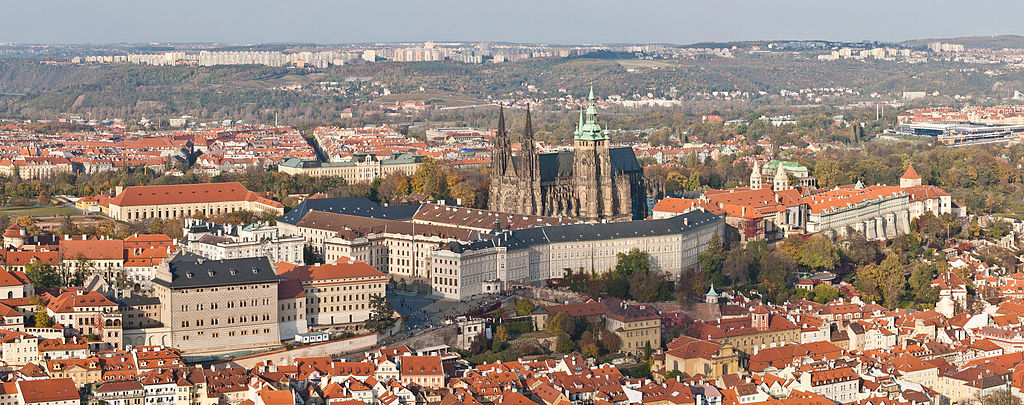
\includegraphics[width=.65\linewidth, trim=0 20 0 0, clip]{prague}

  \bigskip

  {\Large\bf Post-Conference Proceedings, Fundamenta Informaticae}
\end{center}

\begin{multicols}{2}
  Since 1994, the RAMICS conference series has been the main venue for
  research on relation algebras, Kleene algebras and similar algebraic
  formalisms, and their applications as conceptual and methodological
  tools in computer science and beyond.

  \medskip

  Theoretical aspects include semigroups, residuated lattices,
  semirings, Kleene algebras, relation algebras, quantales and other
  algebras; their connections with program logics and other logics;
  their use in the theories of automata, concurrency, formal
  languages, games, networks and programming languages; the
  development of algebraic, algorithmic, category-theoretic,
  coalgebraic and proof-theoretic methods for these theories; their
  formalisation with theorem provers.

  \medskip

  Applications include tools and techniques for program correctness,
  specification and verification; quantitative and qualitative models
  and semantics of computing systems and processes; algorithm design,
  automated reasoning, network protocol analysis, social choice,
  optimisation and control.

  \bigskip

  \hfill {\Large \bf Open Call for Papers}

  \medskip

  The \textbf{Fundamenta Informaticae} journal has kindly agreed to
  publish a Special Issue devoted to the themes of the RAMiCS
  conferences. This follows up on RAMiCS 2024 which was held in
  Prague, collocated with AiML, in August. We are calling for
  contributions based on the presentations at RAMiCS 2024, but the
  special issue is open to papers which are related to the themes of
  the conference without having been presented at RAMiCS 2024.

  We are calling for submission of original work not published or
  under review for publication elsewhere. The submission may or may
  not be based on a previous contribution to RAMiCS 2024. All articles
  submitted to this special issue will undergo the usual rigorous
  reviewing process of Fundamenta Informaticae, which will be
  coordinated by the guest editors.
  
  \bigskip
  
  \hfill {\Large \bf Important Dates}

  \medskip

  The projected deadline for the special issue is \textbf{15 April
    2025}, but we would appreciate if you could announce your
  intention to submit a paper as soon as possible. We intend to
  publish the special issue by April 2027.

  \bigskip
  
  \hfill {\Large \bf Guest Editors}

  \medskip

  \textbf{Uli Fahrenberg}, EPITA Rennes, France

  \hfill \texttt{uli.fahrenberg@epita.fr}
  
  \textbf{Wesley Fussner}, Institute of Computer Science of the Czech
  Academy of Sciences, Prague, Czechia

  \hfill \texttt{fussner@cs.cas.cz}

  \textbf{Roland Glück}, German Aerospace Center, Augsburg, Germany
  \hfill \texttt{Roland.Glueck@dlr.de}

  \bigskip
  \hfill
  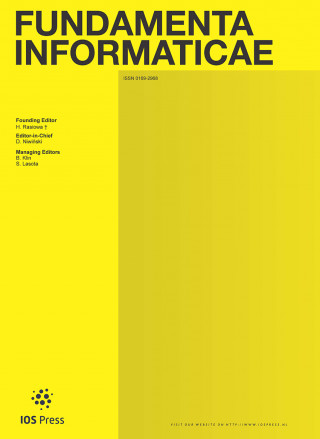
\includegraphics[width=.65\linewidth]{fi}
\end{multicols}

\smallskip

\begin{center}
  {\Huge https://ramics-conf.github.io/2024/}
\end{center}


%\vspace*{-2ex}

\end{document}
